\documentclass[12pt,reqno]{amsart}
\usepackage{/Users/johnmyers/GoogleDrive/tex/handout,/Users/johnmyers/GoogleDrive/tex/customcommands,polynom}
\usepackage{caption}

\hdr{MAT 240}{\S16.3 Triple integrals}

\begin{document}

\textbf{Suggested problems:} 1-51 odd

\bigskip
\hrule

\bigskip
\vspace{-0.1in}
\prob For each part below, set up the integral $\int_W f(x,y,z) \ dV$ where $W$ is the region of $xyz$-space shown.

\bigskip
\begin{enumerate}
\item\textcolor{white}{blank} \\

\includegraphics[scale=1]{1.pdf} \textcolor{red}{$\displaystyle\int_{-2}^2 \int_0^{4-y^2} \int_0^x f(x,y,z) \ dz dxdy$}
\item\textcolor{white}{blank} \\

\includegraphics[scale=1]{2.pdf} \textcolor{red}{$\displaystyle\int_0^1 \int_0^1 \int_0^{xy} f(x,y,z) \ dz dxdy$}
\item\textcolor{white}{blank} \\
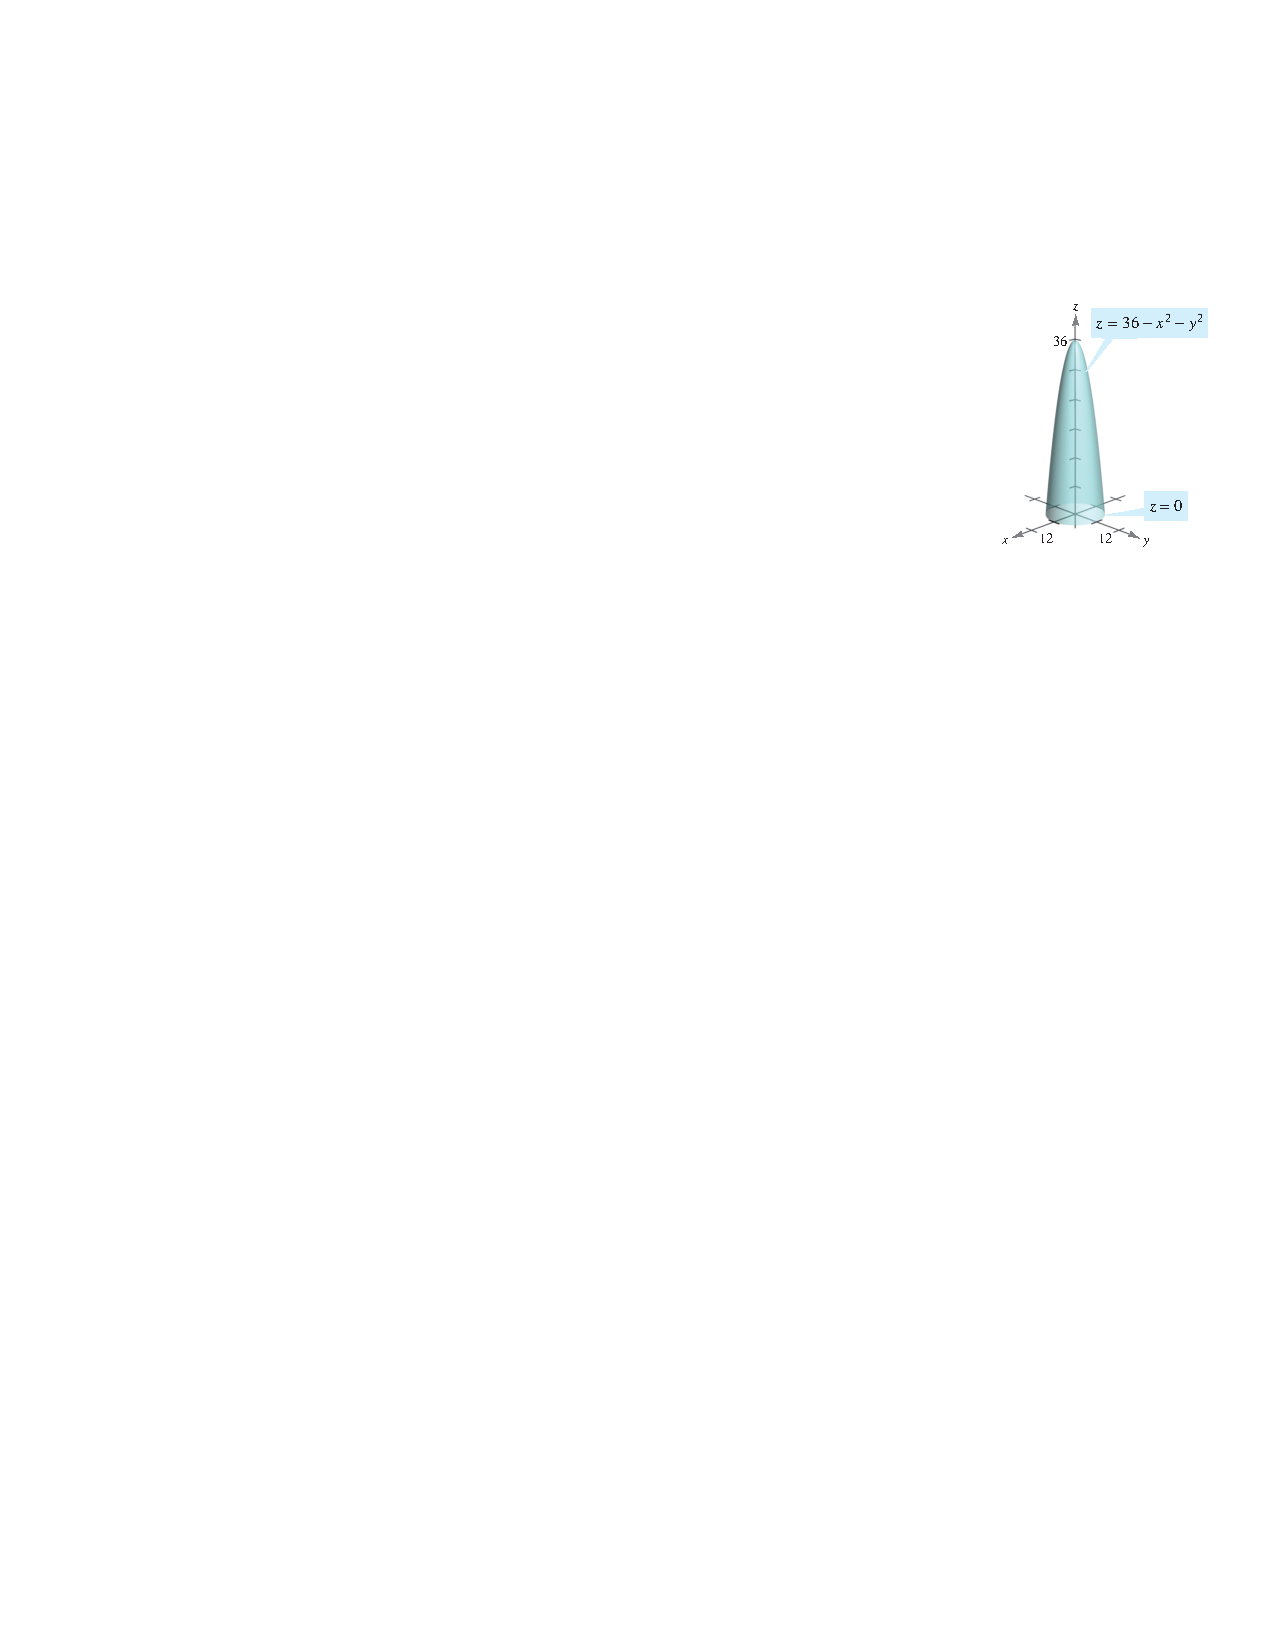
\includegraphics[scale=1]{4.pdf} \textcolor{red}{$\displaystyle\int_{-6}^6 \int_{-\sqrt{36-x^2}}^{\sqrt{36-x^2}} \int_0^{36-x^2-y^2} f(x,y,z) \ dz dydx$}
\item\textcolor{white}{blank} \\

\includegraphics[scale=1]{5.pdf} \textcolor{red}{$\displaystyle\int_0^2 \int_0^{4-x^2} \int_0^{4-x^2}  f(x,y,z) \ dz dydx$}
\item\textcolor{white}{blank} \\

\includegraphics[scale=1]{6.pdf} \textcolor{red}{$\displaystyle\int_0^2 \int_0^{-x+2} \int_0^{9-x^2}  f(x,y,z) \ dz dydx$}
\item\textcolor{white}{blank} \\

\includegraphics[scale=1]{3.pdf} \textcolor{red}{$\displaystyle\int_{-a}^a \int_{-\sqrt{a^2-x^2}}^{\sqrt{a^2-x^2}} \int_{-\sqrt{a^2-x^2-y^2}}^{\sqrt{a^2-x^2-y^2}} f(x,y,z) \ dz dydx$}
\end{enumerate}

\bigskip
\prob For each part below, sketch the region of integration.

\begin{enumerate}
\item $\displaystyle \int_0^1 \int_{-1}^1 \int_0^{\sqrt{1-x^2}} f(x,y,z) \ dz  dx  dy$ \textcolor{red}{See class notes.}
\item $\displaystyle \int_{-1}^1 \int_0^1 \int_{-\sqrt{1-z^2}}^{\sqrt{1-z^2}} f(x,y,z) \ dy dz  dx$ \textcolor{red}{See class notes.}
\item $\displaystyle \int_{0}^1 \int_{-\sqrt{1-z^2}}^{\sqrt{1-z^2}}\int_0^{\sqrt{1-x^2-z^2}} f(x,y,z) \ dy  dx  dz$ \textcolor{red}{See class notes.}
\end{enumerate}

\end{document}